\documentclass[10pt,aspectratio=169]{beamer}

% ==================== PACKAGES ====================
\usepackage[utf8]{inputenc}
\usepackage[T1]{fontenc}
\usepackage{graphicx}
\usepackage{booktabs}
\usepackage{amsmath, amssymb}
\usepackage{tikz}
\usepackage{xcolor}
\usepackage{tabularx}
\usepackage{array}
\usetikzlibrary{shapes, arrows.meta, positioning, fit, backgrounds, calc, shadows}

% ==================== THEME AND COLORS ====================
\usetheme{Madrid}
\usecolortheme{whale}

% Define custom academic color palette
\definecolor{primaryblue}{RGB}{25, 65, 110}
\definecolor{accentteal}{RGB}{0, 130, 130}
\definecolor{accentorange}{RGB}{215, 95, 30}
\definecolor{darkgrey}{RGB}{60, 60, 60}
\definecolor{lightgrey}{RGB}{240, 240, 240}
\definecolor{midgrey}{RGB}{180, 180, 180}
\definecolor{softgreen}{RGB}{40, 130, 90}

% Apply custom colors to beamer elements
\setbeamercolor{structure}{fg=primaryblue}
\setbeamercolor{frametitle}{bg=primaryblue, fg=white}
\setbeamercolor{section in toc}{fg=primaryblue}
\setbeamercolor{block title}{bg=primaryblue, fg=white}
\setbeamercolor{block body}{bg=lightgrey, fg=darkgrey}
\setbeamercolor{block title alerted}{bg=accentorange, fg=white}
\setbeamercolor{block body alerted}{bg=lightgrey, fg=darkgrey}
\setbeamercolor{block title example}{bg=accentteal, fg=white}
\setbeamercolor{block body example}{bg=lightgrey, fg=darkgrey}
\setbeamercolor{itemize item}{fg=primaryblue}
\setbeamercolor{itemize subitem}{fg=accentteal}
\setbeamercolor{section in head/foot}{bg=primaryblue, fg=white}
\setbeamercolor{subsection in head/foot}{bg=primaryblue!80, fg=white}

% Frame title styling
\setbeamerfont{frametitle}{size=\large, series=\bfseries}
\setbeamertemplate{frametitle}[default][left]
\setbeamertemplate{navigation symbols}{}
\setbeamertemplate{footline}[frame number]

% ==================== DOCUMENT ====================
\begin{document}

% ---------- CUSTOM TITLE SLIDE (visible colors, no theme titlepage) ----------
\begin{frame}[plain]
\begin{tikzpicture}[remember picture, overlay]
  % Title band (blue) and orange divider, anchored to page north
  \fill[primaryblue] ([yshift=-0.9cm]current page.north west) rectangle ([yshift=-2.7cm]current page.north east);
  \fill[accentorange] ([yshift=-2.7cm]current page.north west) rectangle ([yshift=-2.85cm]current page.north east);
  % Bottom date band (blue)
  \fill[primaryblue] ([yshift=1.4cm]current page.south west) rectangle ([yshift=0cm]current page.south east);

  % Title text (centered inside the blue band)
  \node[anchor=center, text=white, align=center, font=\normalsize\bfseries,
        text width=0.9\paperwidth]
        at ([yshift=-1.8cm]current page.north)
        {Parameter-Efficient Adaptation of SAM 2 \\ for Sentinel-1 SAR Flood Mapping in Bangladesh};

  % Subtitle, positioned below the orange divider with a clear gap
  \node[anchor=north, text=primaryblue, align=center, font=\small\itshape,
        text width=0.9\paperwidth]
        at ([yshift=-3.2cm]current page.north)
        {A Literature Review and Project Proposal};

  % Authors block, well clear of the subtitle
  \node[anchor=north, text=darkgrey, align=center, font=\footnotesize,
        text width=0.9\paperwidth]
        at ([yshift=-4.6cm]current page.north) {%
    \textbf{\normalsize Aksan Gony Alif \quad Mahbubur Rahman} \\[0.4em]
    Department of Computer Science and Engineering \\
    BRAC University, Dhaka, Bangladesh
  };

  % Project context line, with breathing room above the date band
  \node[anchor=south, text=darkgrey, align=center, font=\scriptsize\itshape,
        text width=0.9\paperwidth]
        at ([yshift=1.7cm]current page.south)
        {Computer Vision Project: Literature Review Presentation};

  % Date inside the bottom blue band
  \node[anchor=center, text=white, font=\small]
        at ([yshift=0.7cm]current page.south) {\today};
\end{tikzpicture}
\end{frame}

% ==================== SECTION 1: MOTIVATION ====================
\section{Motivation}

\begin{frame}{The Problem: Bangladesh Floods Every Year}
\begin{columns}[T,onlytextwidth]
\column{0.55\textwidth}
\textbf{The reality on the ground:}
\begin{itemize}
\item 20 to 25\% of Bangladesh inundates in typical monsoons; 30 to 60\% in severe years
\item 2022 Sylhet flood: 7.2 million affected, $\sim$480{,}000 displaced to shelters
\item Ganges-Brahmaputra-Meghna delta: world's largest delta system
\end{itemize}

\vspace{0.5em}
\textbf{What's needed:}
\begin{itemize}
\item Rapid, accurate flood-extent maps
\item Available within hours, not days
\item Reliable in any weather condition
\end{itemize}

\column{0.45\textwidth}
\begin{block}{Operational stakes}
Better flood maps directly translate into:
\begin{itemize}
\item Faster boat dispatch to villages
\item Smarter relief truck routing
\item Faster damage assessment
\item Lives saved
\end{itemize}
\end{block}
\end{columns}
\end{frame}

\begin{frame}{Why Satellites? And Why Radar Specifically?}
\begin{columns}[T,onlytextwidth]
\column{0.5\textwidth}
\textbf{\textcolor{accentorange}{Optical Satellites (Sentinel-2)}}
\begin{itemize}
\item RGB-like multispectral imagery
\item Easy to interpret visually
\item \textbf{Useless during monsoon}
\item Clouds block visible/IR light
\item Cloud cover $>80\%$ for weeks
\end{itemize}

\column{0.5\textwidth}
\textbf{\textcolor{softgreen}{Radar Satellites (Sentinel-1)}}
\begin{itemize}
\item Synthetic Aperture Radar (SAR)
\item \textbf{Sees through clouds, day/night}
\item Free, global, 6-day revisit
\item 10m spatial resolution
\item Dual-polarization (VV + VH)
\end{itemize}
\end{columns}

\vspace{0.8em}
\begin{center}
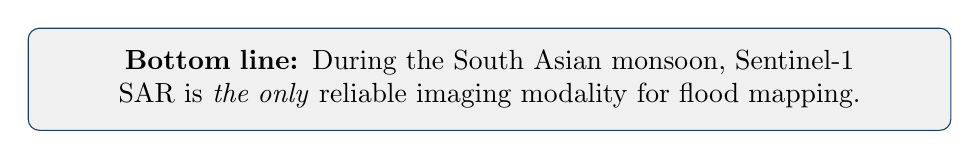
\begin{tikzpicture}
\node[rectangle, draw=primaryblue, fill=lightgrey, rounded corners,
      inner sep=8pt, text width=0.92\linewidth, align=center] (box) {%
\textbf{Bottom line:} During the South Asian monsoon, Sentinel-1 SAR is \textit{the only} reliable imaging modality for flood mapping.};
\end{tikzpicture}
\end{center}
\end{frame}

\begin{frame}{But SAR is Hard for Computer Vision}
\begin{columns}[T,onlytextwidth]
\column{0.5\textwidth}
\textbf{What makes SAR different:}
\begin{itemize}
\item Speckle noise (multiplicative, not additive)
\item Only 1 or 2 channels (not 3-channel RGB)
\item Logarithmic dB scale, wide dynamic range
\item Water = dark (specular reflection)
\item Vegetation, buildings = bright (backscatter)
\end{itemize}

\column{0.5\textwidth}
\textbf{Why this breaks foundation models:}
\begin{itemize}
\item Pretrained on natural RGB photos
\item Never seen radar imagery
\item Statistics are alien
\item Zero-shot performance: poor
\end{itemize}
\end{columns}

\vspace{0.5em}
\begin{alertblock}{The opportunity}
\textbf{Adapt} a powerful foundation model (Segment Anything Model 2) to this new modality \textbf{efficiently}, without millions of dollars of compute.
\end{alertblock}
\end{frame}

\begin{frame}{Our Four Research Questions}
\begin{enumerate}
\item[\textbf{RQ1}] \textbf{Adaptation method:} Which parameter-efficient fine-tuning (PEFT) approach works best for SAM 2 on Sentinel-1 SAR?

\vspace{0.3em}
\item[\textbf{RQ2}] \textbf{Polarimetric prompts:} How should we compose the dual-polarization channels (VV, VH) into the 3-channel input SAM expects?

\vspace{0.3em}
\item[\textbf{RQ3}] \textbf{Confidence:} Can we add calibrated uncertainty estimates to flood maps for operational decision support?

\vspace{0.3em}
\item[\textbf{RQ4}] \textbf{Generalization:} Does a globally-trained model work on the Ganges-Brahmaputra delta specifically?
\end{enumerate}
\end{frame}

% ==================== SECTION 2: CONFERENCE PAPERS ====================
\section{Reviewed: A*/A Conference Papers}

\begin{frame}{Paper 1 \quad Segment Anything (SAM)}
\begin{block}{Citation}
Kirillov, A., Mintun, E., Ravi, N., \textit{et al.} (2023). \textbf{Segment Anything}. \textit{ICCV 2023} (Best Paper Honorable Mention). pp. 4015 to 4026. \\
\textcolor{primaryblue}{arXiv:2304.02643} \quad $\sim$17{,}000 citations
\end{block}

\begin{columns}[T,onlytextwidth]
\column{0.5\textwidth}
\textbf{What they did:}
\begin{itemize}
\item Built a foundation model for segmentation
\item 3 components: image encoder (ViT), prompt encoder, mask decoder
\item Created SA-1B: 1 billion masks, 11M images
\item Released as open weights (Apache 2.0)
\end{itemize}

\column{0.5\textwidth}
\textbf{Key innovations:}
\begin{itemize}
\item Promptable segmentation as a task
\item Data engine with model-in-the-loop
\item Strong zero-shot generalization
\item Single model, many downstream tasks
\end{itemize}
\end{columns}

\vspace{0.5em}
\begin{alertblock}{Relevance to our project}
\textbf{This is our starting point.} We adapt SAM (and its successor) to SAR flood mapping. Without SAM, no foundation-model-based approach exists for our task.
\end{alertblock}
\end{frame}

\begin{frame}{Paper 2 \quad SAM 2: Segment Anything in Images and Videos}
\begin{block}{Citation}
Ravi, N., Gabeur, V., Hu, Y.-T., \textit{et al.} (2025). \textbf{SAM 2: Segment Anything in Images and Videos}. \textit{ICLR 2025 (Oral)}. \\
\textcolor{primaryblue}{arXiv:2408.00714} \quad $\sim$2{,}700+ citations
\end{block}

\begin{columns}[T,onlytextwidth]
\column{0.5\textwidth}
\textbf{Three big upgrades over SAM:}
\begin{itemize}
\item \textbf{Hiera encoder}: multi-scale features
\item \textbf{Memory module}: streaming attention across frames
\item \textbf{6$\times$ faster, more accurate}: even on still images
\end{itemize}

\column{0.5\textwidth}
\textbf{Model variants (open weights):}
\begin{itemize}
\item Hiera-Tiny: 39M parameters
\item Hiera-Small: 46M
\item \textbf{Hiera-Base+: 81M (our choice)}
\item Hiera-Large: 224M
\end{itemize}
\end{columns}

\vspace{0.5em}
\begin{alertblock}{Relevance to our project}
\textbf{This is our chosen backbone.} The memory module is a hidden gem: it was designed for video, but it perfectly handles \textbf{pre-flood vs.\ post-flood image pairs}, exactly the bi-temporal structure of SAR flood detection.
\end{alertblock}
\end{frame}

\begin{frame}{Paper 3 \quad Conv-LoRA: Convolution Meets LoRA}
\begin{block}{Citation}
Zhong, Z., Tang, Z., He, T., Fang, H., Yuan, C. (2024). \\
\textbf{Convolution Meets LoRA: Parameter Efficient Finetuning for Segment Anything Model}. \\
\textit{ICLR 2024}. \quad \textcolor{primaryblue}{arXiv:2401.17868}
\end{block}

\begin{columns}[T,onlytextwidth]
\column{0.5\textwidth}
\textbf{The core idea:}
\begin{itemize}
\item Standard LoRA $=$ low-rank linear updates
\item Add ultra-light \textit{convolutional} layers
\item Inject \textbf{locality bias} into ViT encoder
\item Trains $<$5\% of model parameters
\end{itemize}

\column{0.5\textwidth}
\textbf{Why convolutions matter:}
\begin{itemize}
\item Plain ViT lacks spatial locality
\item Speckle in SAR is \textit{very} local
\item Water boundaries are local
\item Convolutions match the inductive bias
\end{itemize}
\end{columns}

\vspace{0.5em}
\begin{alertblock}{Relevance to our project}
\textbf{This is our methodology blueprint.} Conv-LoRA was tested on \textit{remote sensing} and \textit{medical imaging}, both domains where SAM's plain ViT struggles. SAR sits squarely in this category.
\end{alertblock}
\end{frame}

\begin{frame}{Conference Papers: At-a-Glance Comparison}
\renewcommand{\arraystretch}{1.4}
\begin{tabularx}{\textwidth}{p{2.4cm} p{2.6cm} p{2.4cm} X}
\toprule
\textbf{Paper} & \textbf{Venue (Tier)} & \textbf{Year} & \textbf{Role in Our Project} \\
\midrule
SAM \cite{Kirillov2023SAM} & ICCV (A*) & 2023 & Foundation model we adapt \\
SAM 2 \cite{Ravi2025SAM2} & ICLR Oral (A*) & 2025 & Chosen backbone plus memory module for bi-temporal SAR \\
Conv-LoRA \cite{Zhong2024ConvLoRA} & ICLR (A*) & 2024 & Adaptation method blueprint \\
\bottomrule
\end{tabularx}

\vspace{1em}
\begin{exampleblock}{Narrative arc}
\textbf{Foundation} (SAM) $\rightarrow$ \textbf{Upgrade} (SAM 2) $\rightarrow$ \textbf{Method} (Conv-LoRA). \\ Three papers, three roles, one coherent technical foundation.
\end{exampleblock}
\end{frame}

% ==================== SECTION 3: JOURNAL PAPERS ====================
\section{Reviewed: Q1 Journal Papers}

\begin{frame}{Paper 4 \quad MedSAM: Segment Anything in Medical Images}
\begin{block}{Citation}
Ma, J., He, Y., Li, F., Han, L., You, C., Wang, B. (2024). \\
\textbf{Segment Anything in Medical Images}. \\
\textit{Nature Communications}, 15, 654. \quad \textcolor{primaryblue}{IF: 15.7 (Q1, Multidisciplinary Sciences)}
\end{block}

\begin{columns}[T,onlytextwidth]
\column{0.5\textwidth}
\textbf{What they did:}
\begin{itemize}
\item Adapted SAM to medical imaging
\item Curated 1.57M mask annotations
\item Spans CT, MRI, ultrasound, X-ray, microscopy
\item Bounding-box-prompted segmentation
\item Released model and dataset publicly
\end{itemize}

\column{0.5\textwidth}
\textbf{Why this is the gold-standard template:}
\begin{itemize}
\item First major SAM adaptation to a non-RGB modality
\item Showed: pretrained features \textit{do} transfer
\item Validated by $\sim$2{,}800 citations
\item Published in a top-IF journal
\end{itemize}
\end{columns}

\vspace{0.5em}
\begin{alertblock}{Relevance to our project}
\textbf{This is the writeup template our committee will recognize.} The story of ``adapt SAM to a domain it was never designed for'' is now well-established. We replicate the framing for SAR using PEFT instead of full fine-tuning.
\end{alertblock}
\end{frame}

\begin{frame}{Paper 5 \quad DAM-Net: ViT for SAR Flood Detection}
\begin{block}{Citation}
Saleh, T., Weng, X., Holail, S., Hao, C., Xia, G.-S. (2024). \\
\textbf{DAM-Net: Flood detection from SAR imagery using differential attention metric-based vision transformers}. \\
\textit{ISPRS Journal of Photogrammetry and Remote Sensing}, 212, 440 to 453. \quad \textcolor{primaryblue}{JCR 2024 IF: 12.2 (Q1)}
\end{block}

\begin{columns}[T,onlytextwidth]
\column{0.5\textwidth}
\textbf{Architecture:}
\begin{itemize}
\item Siamese Vision Transformer
\item Pre-flood + post-flood SAR pairs
\item Temporal differential fusion module
\item Class token records semantic change
\end{itemize}

\column{0.5\textwidth}
\textbf{Performance on S1GFloods:}
\begin{itemize}
\item F1: \textbf{96.5\%}
\item IoU: \textbf{93.2\%}
\item Released the S1GFloods dataset
\item Current SOTA on bi-temporal SAR
\end{itemize}
\end{columns}

\vspace{0.5em}
\begin{alertblock}{Relevance to our project}
\textbf{This is the SOTA non-foundation-model baseline we must beat (or come close to).} DAM-Net validates the bi-temporal Siamese architecture, which we replicate using SAM 2's memory module instead of an explicit Siamese network.
\end{alertblock}
\end{frame}

\begin{frame}{Paper 6 \quad ClassWise-SAM-Adapter (CWSAM)}
\begin{block}{Citation}
Pu, X., Jia, H., Zheng, L., Wang, F., Xu, F. (2025). \\
\textbf{ClassWise-SAM-Adapter: Parameter-Efficient Fine-Tuning Adapts Segment Anything to SAR Domain for Semantic Segmentation}. \\
\textit{IEEE J. Selected Topics in Applied Earth Observations and Remote Sensing}, 18, 4791 to 4806. \quad \textcolor{primaryblue}{(Q1)}
\end{block}

\begin{columns}[T,onlytextwidth]
\column{0.5\textwidth}
\textbf{What they did:}
\begin{itemize}
\item Froze most of SAM's parameters
\item Added lightweight adapters to encoder
\item Built a class-aware mask decoder
\item Frequency-domain task-specific input
\item \textbf{Target: SAR landcover classification}
\end{itemize}

\column{0.5\textwidth}
\textbf{Why it matters and how we differ:}
\begin{itemize}
\item \textcolor{accentorange}{Same:} SAM + adapter + SAR
\item \textcolor{softgreen}{Different:} flood mapping (not landcover)
\item \textcolor{softgreen}{Different:} SAM 2 (not SAM v1)
\item \textcolor{softgreen}{Different:} confidence-aware
\item \textcolor{softgreen}{Different:} Bangladesh test set
\end{itemize}
\end{columns}

\vspace{0.5em}
\begin{alertblock}{Relevance to our project}
\textbf{This is our nearest neighbor in the literature.} Our four differentiators above are precisely the \textbf{novelty wedge} that distinguishes our thesis from CWSAM.
\end{alertblock}
\end{frame}

\begin{frame}{Journal Papers: At-a-Glance Comparison}
\renewcommand{\arraystretch}{1.4}
\begin{tabularx}{\textwidth}{p{2.4cm} p{3.2cm} p{1.4cm} X}
\toprule
\textbf{Paper} & \textbf{Journal (IF, Quartile)} & \textbf{Year} & \textbf{Role in Our Project} \\
\midrule
MedSAM \cite{Ma2024MedSAM} & Nat.\ Comm.\ (15.7, Q1) & 2024 & Cross-domain adaptation template \\
DAM-Net \cite{Saleh2024DAMNet} & ISPRS-J P\&RS (12.2, Q1) & 2024 & Non-FM SOTA baseline to beat \\
CWSAM \cite{Pu2025CWSAM} & IEEE J-STARS (Q1) & 2025 & Closest prior work; novelty wedge \\
\bottomrule
\end{tabularx}

\vspace{1em}
\begin{exampleblock}{Narrative arc}
\textbf{How to write up} (MedSAM) $\rightarrow$ \textbf{What to beat} (DAM-Net) $\rightarrow$ \textbf{What we extend} (CWSAM). \\
Together with the conference papers, we have a complete view of the field.
\end{exampleblock}
\end{frame}

% ==================== SECTION 4: SYNTHESIS ====================
\section{Research Gap and Synthesis}

\begin{frame}{The Research Gap, Visualized}
\begin{center}
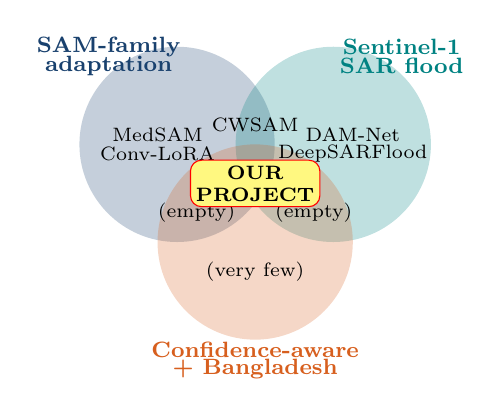
\begin{tikzpicture}[scale=0.62]
\fill[primaryblue, opacity=0.25] (-1.6,0) circle (2.0cm);
\fill[accentteal, opacity=0.25] (1.6,0) circle (2.0cm);
\fill[accentorange, opacity=0.25] (0,-2.0) circle (2.0cm);

\node[primaryblue, font=\bfseries\footnotesize] at (-3.0,2.0) {SAM-family};
\node[primaryblue, font=\bfseries\footnotesize] at (-3.0,1.6) {adaptation};
\node[accentteal, font=\bfseries\footnotesize] at (3.0,2.0) {Sentinel-1};
\node[accentteal, font=\bfseries\footnotesize] at (3.0,1.6) {SAR flood};
\node[accentorange, font=\bfseries\footnotesize] at (0,-4.2) {Confidence-aware};
\node[accentorange, font=\bfseries\footnotesize] at (0,-4.6) {+ Bangladesh};

\node[font=\scriptsize] at (-2.0,0.2) {MedSAM};
\node[font=\scriptsize] at (-2.0,-0.2) {Conv-LoRA};
\node[font=\scriptsize] at (2.0,0.2) {DAM-Net};
\node[font=\scriptsize] at (2.0,-0.2) {DeepSARFlood};
\node[font=\scriptsize] at (0,-2.6) {(very few)};

\node[font=\scriptsize, align=center] at (0,0.4) {CWSAM};
\node[font=\scriptsize, align=center] at (-1.2,-1.4) {(empty)};
\node[font=\scriptsize, align=center] at (1.2,-1.4) {(empty)};

\node[draw=red, fill=yellow!50, rounded corners, font=\bfseries\scriptsize, align=center, inner sep=2pt] at (0,-0.8) {\textbf{OUR}\\ \textbf{PROJECT}};

\end{tikzpicture}
\end{center}

\vspace{0.5em}
\begin{exampleblock}{The triple intersection is empty, and that's our contribution}
No published peer-reviewed work combines all three: \textbf{SAM-family adaptation} $\cap$ \textbf{Sentinel-1 SAR flood mapping} $\cap$ \textbf{confidence-aware regional benchmark.}
\end{exampleblock}
\end{frame}

% ==================== SECTION 5: PROPOSED APPROACH ====================
\section{Proposed Approach}

\begin{frame}{End-to-End Pipeline}
\begin{center}
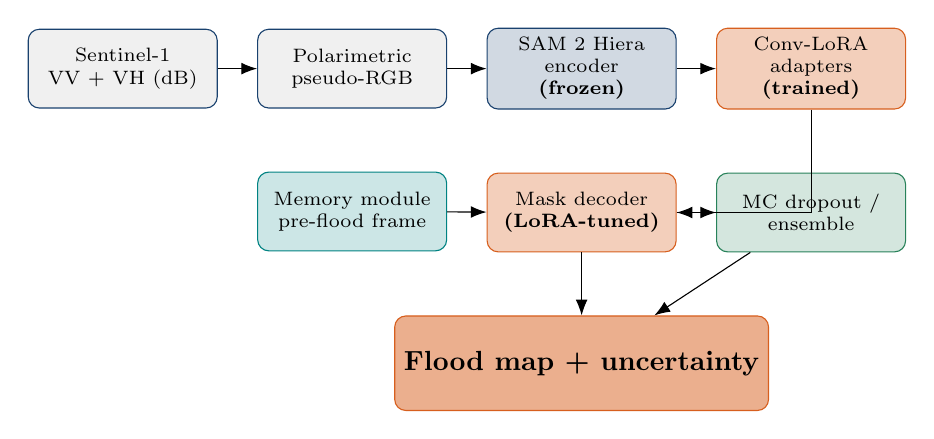
\begin{tikzpicture}[node distance=0.5cm, every node/.style={font=\scriptsize}]
\node[rectangle, draw=primaryblue, fill=lightgrey, rounded corners, minimum width=2.4cm, minimum height=1cm, align=center] (input) {Sentinel-1 \\ VV + VH (dB)};
\node[rectangle, draw=primaryblue, fill=lightgrey, rounded corners, minimum width=2.4cm, minimum height=1cm, align=center, right=of input] (poly) {Polarimetric \\ pseudo-RGB};
\node[rectangle, draw=primaryblue, fill=primaryblue!20, rounded corners, minimum width=2.4cm, minimum height=1cm, align=center, right=of poly] (enc) {SAM 2 Hiera \\ encoder \\ \textbf{(frozen)}};
\node[rectangle, draw=accentorange, fill=accentorange!30, rounded corners, minimum width=2.4cm, minimum height=1cm, align=center, right=of enc] (peft) {Conv-LoRA \\ adapters \\ \textbf{(trained)}};
\node[rectangle, draw=accentteal, fill=accentteal!20, rounded corners, minimum width=2.4cm, minimum height=1cm, align=center, below=0.8cm of poly] (mem) {Memory module \\ pre-flood frame};
\node[rectangle, draw=accentorange, fill=accentorange!30, rounded corners, minimum width=2.4cm, minimum height=1cm, align=center, below=0.8cm of enc] (dec) {Mask decoder \\ \textbf{(LoRA-tuned)}};
\node[rectangle, draw=softgreen, fill=softgreen!20, rounded corners, minimum width=2.4cm, minimum height=1cm, align=center, below=0.8cm of peft] (conf) {MC dropout / \\ ensemble};
\node[rectangle, draw=accentorange, fill=accentorange!50, rounded corners, minimum width=4cm, minimum height=1.2cm, align=center, below=0.8cm of dec, font=\bfseries] (out) {Flood map + uncertainty};

\draw[-{Latex[length=2mm]}] (input) -- (poly);
\draw[-{Latex[length=2mm]}] (poly) -- (enc);
\draw[-{Latex[length=2mm]}] (enc) -- (peft);
\draw[-{Latex[length=2mm]}] (peft) |- (dec);
\draw[-{Latex[length=2mm]}] (mem) -- (dec);
\draw[-{Latex[length=2mm]}] (dec) -- (conf);
\draw[-{Latex[length=2mm]}] (conf) -- (out);
\draw[-{Latex[length=2mm]}] (dec) -- (out);
\end{tikzpicture}
\end{center}

\vspace{0.5em}
\begin{exampleblock}{Key design choices}
Frozen pretrained encoder + trainable Conv-LoRA adapters + SAM 2 memory module for bi-temporal context + Monte-Carlo dropout for calibrated uncertainty.
\end{exampleblock}
\end{frame}

\begin{frame}{Methodology: Four Experimental Pillars}
\setlength{\leftmargini}{1.8cm}
\begin{enumerate}
\item[\textbf{Pillar 1}] \textbf{PEFT comparison:} 4 methods (LoRA, DoRA, Conv-LoRA, AdaptFormer) $\times$ 2 backbones (SAM ViT-B, SAM 2 Hiera-B+) $\times$ 3 seeds = \textbf{24 runs}

\vspace{0.3em}
\item[\textbf{Pillar 2}] \textbf{Polarimetric prompt ablation:} 3 channel compositions
\begin{itemize}
\item[\scriptsize$\circ$] (VV, VH, VV/VH ratio): industry convention
\item[\scriptsize$\circ$] (VV, VH, VV$-$VH difference): physically interpretable
\item[\scriptsize$\circ$] (VV, VV, VV): single-pol control
\end{itemize}

\vspace{0.3em}
\item[\textbf{Pillar 3}] \textbf{Confidence-aware mechanism:} Monte Carlo dropout (20 passes) or 5-seed deep ensemble; calibration via expected calibration error and reliability diagrams

\vspace{0.3em}
\item[\textbf{Pillar 4}] \textbf{Out-of-distribution generalization:} Sen1Floods11 hand-labeled test $\rightarrow$ \textbf{Bolivia held-out split} (the only truly held-out country in Sen1Floods11)
\end{enumerate}
\end{frame}

\begin{frame}{Datasets We Will Use}
\renewcommand{\arraystretch}{1.3}
\footnotesize
\begin{tabularx}{\textwidth}{p{3.0cm} p{2.3cm} p{1.3cm} X}
\toprule
\textbf{Dataset} & \textbf{Use} & \textbf{Size} & \textbf{Notes} \\
\midrule
Sen1Floods11 hand & Train, val, in-dist test & 700 MB & 446 hand-labeled chips across 10 countries; canonical SAR flood benchmark \\
Sen1Floods11 Bolivia & OOD held-out test & subset of above & 15 chips; only truly held-out country, used by virtually every paper in the area \\
\bottomrule
\end{tabularx}

\vspace{1em}
\begin{alertblock}{Released alongside this thesis}
A \textbf{Bangladesh-2022-Sylhet dataset construction pipeline} (UNOSAT + Copernicus GFM + optional Charter 762) ships as a standalone artifact with empirical evaluation deferred. The \textbf{Pakistan-2022} test set (58 chips, TU Wien labels + Microsoft Planetary Computer Sentinel-1 RTC) is empirically evaluated in this thesis as the strict out-of-distribution slice.
\end{alertblock}
\end{frame}

% ==================== SECTION 6: PLAN ====================
\section{Plan and Expected Contributions}

\begin{frame}{12-Week Project Timeline}
\renewcommand{\arraystretch}{1.2}
\begin{tabularx}{\textwidth}{p{1.4cm} X}
\toprule
\textbf{Weeks} & \textbf{Activities} \\
\midrule
1 to 2 & Literature consolidation, environment setup, sanity-check inference \\
3 & Sen1Floods11 download, PyTorch Dataset class, augmentation pipeline \\
4 & \textbf{Bangladesh-2022-Sylhet test set construction} \\
5 & U-Net baseline reproduction, zero-shot SAM baseline, locked protocol \\
6 to 7 & \textbf{Core PEFT comparison: 4 methods, 2 backbones, 3 seeds} \\
8 & Polarimetric prompt-engineering ablation \\
9 & \textbf{Confidence-aware mechanism + calibration analysis} \\
10 & Vast.ai final sweep including SAM ViT-L stretch (budget $<$\$25) \\
11 to 12 & Analysis, figures, thesis writeup, presentation prep, repo freeze \\
\bottomrule
\end{tabularx}

\vspace{0.5em}
\begin{block}{Hardware: realistic and on-hand}
RTX 3060 12GB (local) for 95\% of training, plus rented RTX 4090 24GB (Vast.ai, $<$\$25 total) for the final sweep including the largest backbone.
\end{block}
\end{frame}

\begin{frame}{Expected Contributions}
\begin{enumerate}
\item[\textbf{C1}] Systematic empirical comparison of \textbf{4 PEFT methods} on \textbf{2 SAM-family backbones} for Sentinel-1 SAR flood mapping: the first such comparison at peer-reviewed quality.

\vspace{0.3em}
\item[\textbf{C2}] A polarimetric prompt-engineering protocol with a defensible recommendation for composing dual-polarization SAR into 3-channel pseudo-RGB.

\vspace{0.3em}
\item[\textbf{C3}] The \textbf{first application of a confidence-aware mechanism to SAR flood mapping with SAM 2}, with calibration analysis stratified by terrain type.

\vspace{0.3em}
\item[\textbf{C4}] A standalone \textbf{Bangladesh-2022-Sylhet dataset construction pipeline} released alongside the thesis, with empirical evaluation deferred to subsequent work.

\vspace{0.3em}
\item[\textbf{C5}] Open-source release of all code, configurations, and trained models for full reproducibility.
\end{enumerate}
\end{frame}

\begin{frame}{Risks and Mitigations}
\renewcommand{\arraystretch}{1.4}
\begin{tabularx}{\textwidth}{p{4.5cm} X}
\toprule
\textbf{Risk} & \textbf{Mitigation} \\
\midrule
A PEFT method fails to converge & Drop from comparison; report on remaining methods; document the failure as a finding \\
\midrule
Cloud-GPU budget exceeded & Reduce to one backbone and one PEFT method per ablation; mark missing rows as deferred to subsequent work \\
\midrule
Competing work appears during the project & Pivot framing toward strongest distinguishing components: confidence mechanism, released construction pipeline \\
\midrule
Foundation model loses to U-Net (PANGAEA effect) & Report honestly; argue that PEFT closes the compute-efficiency gap even if not the performance gap \\
\bottomrule
\end{tabularx}
\end{frame}

% ==================== SECTION 7: CONCLUSION ====================
\section{Conclusion}

\begin{frame}{Summary: What We Set Out to Do}
\begin{exampleblock}{In one sentence}
We adapt SAM 2 to Sentinel-1 SAR for flood mapping using parameter-efficient fine-tuning, add a confidence-aware mechanism, evaluate on Sen1Floods11 + Bolivia + Pakistan-2022, and release a Bangladesh test set construction pipeline as a standalone artifact.
\end{exampleblock}

\vspace{0.8em}
\textbf{Why it matters:}
\begin{itemize}
\item \textbf{Operational:} Bangladesh and the wider Indo-Gangetic plain need better monsoon flood maps; SAR is the only reliable modality
\item \textbf{Scientific:} Closes a real gap at the intersection of foundation models and SAR remote sensing
\item \textbf{Methodological:} Demonstrates PEFT-based foundation-model adaptation on consumer hardware
\item \textbf{Reproducible:} Open-source pipeline lets future work extend evaluation to regional test sets
\end{itemize}

\vspace{0.5em}
\centering
\textit{Six papers reviewed $\rightarrow$ One coherent project $\rightarrow$ Four defensible contributions.}
\end{frame}

\begin{frame}{References: The Six Reviewed Papers}
\providecommand{\bibsection}{}
\renewcommand{\bibsection}{}
\footnotesize
\begin{thebibliography}{9}
\bibitem{Kirillov2023SAM}
A.\ Kirillov \textit{et al.}, ``Segment Anything,'' \textit{ICCV}, 2023, pp.\ 4015 to 4026. arXiv:2304.02643.

\bibitem{Ravi2025SAM2}
N.\ Ravi \textit{et al.}, ``SAM 2: Segment Anything in Images and Videos,'' \textit{ICLR (Oral)}, 2025. arXiv:2408.00714.

\bibitem{Zhong2024ConvLoRA}
Z.\ Zhong \textit{et al.}, ``Convolution Meets LoRA: Parameter Efficient Finetuning for Segment Anything Model,'' \textit{ICLR}, 2024. arXiv:2401.17868.

\bibitem{Ma2024MedSAM}
J.\ Ma \textit{et al.}, ``Segment Anything in Medical Images,'' \textit{Nature Communications}, 15:654, 2024.

\bibitem{Saleh2024DAMNet}
T.\ Saleh \textit{et al.}, ``DAM-Net: Flood detection from SAR imagery using differential attention metric-based vision transformers,'' \textit{ISPRS Journal of Photogrammetry and Remote Sensing}, 212:440 to 453, 2024.

\bibitem{Pu2025CWSAM}
X.\ Pu \textit{et al.}, ``ClassWise-SAM-Adapter: Parameter-Efficient Fine-Tuning Adapts Segment Anything to SAR Domain for Semantic Segmentation,'' \textit{IEEE J-STARS}, 18:4791 to 4806, 2025.
\end{thebibliography}
\end{frame}

% ---------- THANK YOU SLIDE ----------
\begin{frame}[plain]
\begin{center}
\vfill
{\Huge \textcolor{primaryblue}{\textbf{Thank You}}}
\vfill
\end{center}
\end{frame}

\end{document}
